$\zeta(z)\neq0$ for $\Re(z)\geq1$. \\
We supposed that $\zeta(1+ia)=0$. \\
It follows that $F(z)=\zeta(z)^2\zeta(z+ia)\zeta(z-ia)$ is entire, and for $\Re(z)>1$, $F(z)=\sum_{n=1}^\infty f(n)/n^z$ with each $f(n)\geq0$.

By Landau's Theorem, $F(z)=\sum_{n=1}^\infty\frac{f(n)}{n^z}$ converges absolutely for all $z\in\C$.

For all $z\in\C$,
\[ F(z) = \sum_n \frac{f(n)}{n^z} = \prod_p \paren[\Big]{\frac{1}{1-p^{-z}}}^2 \paren[\Big]{\frac{1}{1-p^{-z-ia}}} \paren[\Big]{\frac{1}{1-p^{-z+ia}}} \]
If we expand and group together the terms involving products of $2$,
\[\sum_{n=2^k} \frac{f(n)}{n^z} = \paren[\Big]{\frac{1}{1-2^{-z}}}^2\paren[\Big]{\frac{1}{1-2^{-z-ia}}}\paren[\Big]{\frac{1}{1-2^{-z+ia}}} \]
In particular, for $z=x>0$, we have
\begin{align*}
F(x) &= \sum_{n=1}^\infty \frac{f(n)}{n^x} \geq \sum_{n=2^k} \frac{f(n)}{n^k} = \frac{1}{(1-2^{-x})^2}\cdot\frac{1}{(1-2^{-x-ia})}\cdot\frac{1}{(1-2^{-x+ia})} \\
&= \frac{1}{(1-2^{-x})^2}\frac{1}{\abs{1-2^{-(x+ia)}}^2} \geq \frac{1}{(1-2^{-x})^2}\cdot\frac{1}{(1+\abs{2^{-(x+ia)}})^2} \\
&= \frac{1}{(1-4^{-x})^2} \to \infty \text{, as $x\to0^+$.}
\end{align*}
This contradicts the fact that $F(z)$ is holomorphic in $\C$ (hence continuous at $0$).

\thm (Newman's Convergence Theorem) \\
Let $\sum_{n=1}^\infty\frac{f(n)}{n^z}$ be a Dirichlet series with $\abs{f(n)}\leq1$ for all $n$.  Suppose $\sum_{n=1}^\infty\frac{f(n)}{n^z}$ converges for $\Re(z)>1$.  Suppose the function
\[ F(z) = \sum_{n=1}^\infty \frac{f(n)}{n^z} \]
(which is holomorphic for $\Re(z)>1$) extends to be holomorphic on some open set $U$ which contains $\set{z}{\Re(z)\geq1}$.  Then $\sum_{n=1}^\infty\frac{f(n)}{n^z}$ converges for $\Re(z)\geq1$. \\
\pf Fix $w$ with $\Re(w)=1$.  Note that $G(z)=F(w+z)$ is holomorphic in $V=U-w=\set{z=u-w}{u\in U}$. \[ \begin{tikzpicture}[scale=1.75]
\path[fill=lightgray](120:0.3)--(240:0.3)arc(-120:120:0.3);
\draw(-1,0)--(2,0);
\draw(0,-1)--(0,1);
\draw(1,-1)--(1,1);
\node[below right]at(1,0){$1$};
\draw[domain=-1:1]plot({1-exp(-\x*\x)/2.5},\x);
\draw[domain=-1:1]plot({1-exp(-\x*\x)/2.5-1},\x);
\draw[decoration={markings,mark=at position 0.25 with {\arrow{>},\node[left]{$\beta$};}},postaction=decorate](120:0.3)--(240:0.3);
\draw[decoration={markings,mark=at position 0.666 with {\arrow{>},\node[above]{$\alpha$};}},postaction=decorate](240:0.3)arc(-120:120:0.3);
\draw[fill](-0.075,-0.15)circle(0.025);
\end{tikzpicture} \] Let $R>1$ and let $r\in(0,\frac12)$ be small enough so that the set
\[ D = \overline{D}(0,R) \cap \set{z}{\Re(z)\geq-r} \]
is contained in $V$.  Let $\gamma$ be the loop which goes once (counterclockwise) around $\partial D$.  Let $\alpha$ be the part of $\gamma$ in $\Re(z)\geq0$ and let $\beta$ be the part in $\Re(z)\leq0$.

We integrate the function
\[ F(w+z) l^z \paren[\Big]{\frac1z+\frac z{R^2}} \]
along $\gamma$ for $l\in\Z^+$.

Note that by Cauchy's Integral Formula
\[ \int_\gamma \frac{F(w+z)l^z}{z} \d z = 2\pi i \cdot F(w+0)l^0 = 2\pi i F(w) \]
and
\[ \int_\gamma \frac{F(w+z)l^z z}{R^2}\d z = 0 \]
so
\begin{align*}
2\pi i F(w) &= \int_\gamma F(w+z)l^z\paren[\Big]{\frac1z+\frac z{R^2}}\d z \\
&= \int_\alpha F(w+z)l^z\paren[\Big]{\frac1z+\frac z{R^2}}\d z + \int_\beta F(w+z)l^z\paren[\Big]{\frac1z+\frac z{R^2}}\d z \\
&= \int_\alpha S_l(w+z)l^z\paren[\Big]{\frac1z+\frac z{R^2}}\d z + \int_\alpha E_l(w+z)l^z\paren[\Big]{\frac1z+\frac z{R^2}}\d z + \int_\beta F(w+z)l^z\paren[\Big]{\frac1z+\frac z{R^2}}\d z
\end{align*}
where for $\Re(z)>0$ we have $F(w+z)=\sum_{n=1}^\infty\frac{f(n)}{n^{w+z}}$ and we write
\begin{align*}
S_l(w+z) &= \sum_{n=1}^l \frac{f(n)}{n^{w+z}} \\
E_l(w+z) &= \sum_{n=l+1}^\infty \frac{f(n)}{n^{w+z}} \\
2\pi i F(w) &= 2\pi i S_l(w) - \int_{-\alpha} S_l(w+z) l^z \paren[\Big]{\frac1z+\frac z{R^2}}\d z + \int_\alpha E_l(w+z)l^z\paren[\Big]{\frac1z+\frac z{R^2}}\d z + \int_\beta F(w+z)l^z\paren[\Big]{\frac1z+\frac z{R^2}}\d z
\end{align*}
since $\int_{(\alpha)(-\alpha)}S_l(w+z)l^z\paren[\big]{\frac1z+\frac z{R^2}}\d z=2\pi iS_l(w)$, as above.

\[ \therefore 2\pi i(F(w)-S_l(w)) = \int_\alpha S_l(w-z)l^{-z}\paren[\Big]{-\frac1z-\frac z{R^2}}\d z + \int_\alpha E_l(w+z)l^z\paren[\Big]{\frac1z+\frac z{R^2}}\d z+\int_\beta F(w+z)l^z\paren[\Big]{\frac1z+\frac z{R^2}}\d z \]
since
\begin{gather*}
\int_{-\alpha}g(z)\d z = \int_{t_1}^{t_2}g(-\alpha(t))\cdot(-\alpha'(t))\d t = -\int_\alpha g(-z)\d z \\
\begin{aligned}
2\pi i(F(w)-S_l(w)) &= A + B \\
\text{where } A &= \int_\alpha(E_l(w+z)l^z-S_l(w-z)l^{-z})\paren[\Big]{\frac1z+\frac z{R^2}}\d z \\
B &= \int_\beta F(w+z) l^z \paren[\Big]{\frac1z+\frac z{R^2}}\d z . \\
\end{aligned} \\
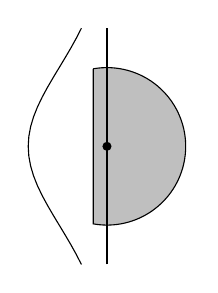
\begin{tikzpicture}
\path[fill=lightgray](100:1)--(-100:1)arc(-100:100:1);
\draw[domain=-1.5:1.5]plot({-exp(-\x*\x/2)},\x);
\draw(100:1)--(-100:1)arc(-100:100:1);
\draw(0,-1.5)--(0,1.5);
\draw[fill](0,0)circle(0.05);
\end{tikzpicture}
\end{gather*}
For $z=x+iy$ on $\alpha$ (so $\abs{z}=R$) with $x>0$
\begin{align*}
\abs[\Big]{\frac1z+\frac z{R^2}} &= \abs[\Big]{\frac{\overline{z}+z}{R^2}} = \frac{2x}{R^2} \\
\abs{E_l(w+z)} &= \abs[\Big]{\sum_{n=l+1}^\infty\frac{f(n)}{n^{w+z}}} \leq \sum_{n=l+1}^\infty \frac{\abs{f(n)}}{\abs{n^{w+z}}} \\
&\leq \sum_{n=l+1}^\infty \frac1{n^{1+x}} \leq \int_l^\infty \frac1{t^{1+x}}\d t \\
&= \brack[\Big]{\frac{-1}{xt^x}}_l^\infty = \frac{1}{xl^x} \\
\abs{S_l(w-z)} &= \abs[\Big]{\sum_{n=1}^l\frac{f(n)}{n^{w-z}}} \\
&\leq \sum_{n=1}^l \frac{1}{n^{1-x}} \\
&= l^{x-1} + \sum_{n=1}^{l-1} n^{x-1} \\
&\leq l^{x-1} + \int_0^l t^{x-1}\d t \\
&= l^{x-1} + \brack[\Big]{\frac{t^x}{x}}_0^l \\
&= l^{x-1} + \frac{l^x}{x} \\
&= l^x\paren[\Big]{\frac1l+\frac1x}
\end{align*}
So we have
\begin{align*}
\abs{A} &\leq \pi R \max_{x+iy\text{ on }\alpha}\paren[\Big]{\frac{1}{xl^x}l^x+l^x\paren[\Big]{\frac1l+\frac1x}l^{-x}}\paren[\Big]{\frac{2x}{R^2}} \\
&= \pi R \max\paren[\Big]{\frac2x+\frac1l}\paren[\Big]{\frac{2x}{R^2}} \\
&= \pi R \max\paren[\Big]{\frac4{R^2}+\frac{2x}{lR^2}} \\
&= \pi R \paren[\Big]{\frac4{R^2}+\frac{2}{lR}} = \frac{4\pi}{R} + \frac{2\pi}{l}
\end{align*}
